% AUTO-GENERATED durch diagram_generator (REV 7.6, TikZ-Bar-Chart)
\begin{tikzpicture}
\begin{axis}[
    ybar,
    bar width=10pt,
    width=0.9500\textwidth,
    height=0.4000\textheight,
    scale only axis,
    title={Comdare-Messvergleich},
    xlabel={Permutation},
    ylabel={Zyklen},
    grid=both,
    enlargelimits=0.05,
    symbolic x coords={ArtComposition\_0,HotComposition\_1,StartComposition\_2,SurfComposition\_3,WormholeComposition\_4,MasstreeComposition\_5},
    xtick=data,
    x tick label style={rotate=45,anchor=east,font=\tiny},
]
\addplot coordinates {
    (ArtComposition\_0,825053.0000)
    (HotComposition\_1,740176.0000)
    (StartComposition\_2,805750.0000)
    (SurfComposition\_3,873976.0000)
    (WormholeComposition\_4,696350.0000)
    (MasstreeComposition\_5,770871.0000)
};
\end{axis}
\end{tikzpicture}
